\chapter{Summary and Outlook} % (fold)
\label{cha:summary_&_outlook}
This thesis covers two broad topics, one based upon the hardware activities and another one based upon the physics analysis. On the hardware front, this thesis includes the studies carried out for the characterization of Gas Electron Multiplier (GEM) detectors for the CMS GE1/1 detector system upgrade, which is followed by the characterisation study of ``\textit{Indian origin}'' GEM foils for the future CMS muon detector system upgrades foreseen during the period 2024-2026. The physics analysis described in this thesis is aimed to measure anomalous Quartic-Gauge Coupling (aQGC) phenomenon using the proton-proton collision data collected using the CMS detector at a center-of-mass energy of 13 \TeV. A brief summary of both these topics task is given below.

For the CMS muon endcap detector system upgrade, triple-layer GEM detectors are proposed to be installed during the Long-Shutdown-2 (2019-2020) period because of their excellent performance capabilities even in the harsh radiation environment conditions at the LHC. This upgrade project is named as CMS GE1/1 upgrade, where the letter “G” stands for GEM, ``E'' stands for End-cap, the first ``1'' corresponds to the first muon station and the second ``1'' corresponds to the first ring of the station. To test the functionality of these GE1/1 detectors, multiple beam tests were carried out in the year 2014 to measure their properties and evaluate their performance in terms of spatial and timing resolution, cluster size and detection efficiency. Results from these beam test campaigns carried out at CERN are documented in this thesis. The detection efficiency of CMS GE1/1 prototype detector, completely instrumented with the proposed readout electronics, is measured using a scintillator and GEM detector based test set-up.

It is observed that the GE1/1 prototype detector has a detection efficiency greater than 98\% and timing resolution is 5-7 ns.

Furthermore, the performance of GE1/1 detectors is scrutinized for two different gas mixtures viz. $Ar:CO_2$ (70:30) and $Ar:CO_2:CF_4$ (40:15:45). It is found that one can operate GEM detectors without $CF_4$, which is a non-eco friendly gas, without compromising the detection efficiency and timing resolution of the detector. To confirm the radiation hardness capabilities of GE1/1 detectors same set of tests were performed on GE1/1 detector, which has been irradiated with gamma rays for long durations. The obtained results were compatible with other GE1/1 detectors thus ensuring their performance in high background rate environments.

Along with the GE1/1 upgrade studies, the characterisation studies of the GEM foil indigenously developed in India were also performed in the Detector laboratory at the University of Delhi. An Indian company, Micropack Pvt. Ltd., developed the technology to develop GEM foils with the help of experts from CERN under the Transfer-of-Technology (TOT) agreement between CERN and India.

GEM foils with dimensions 10 cm $\times$ 10 cm were successfully produced using the double mask technique. These GEM foils are then characterized using optical and electrical methods to check for any defects and abnormalities, which could affect the detector performance. Minimal defects were found in the GEM foils ($<$ 0.13\% of total GEM holes) and a very small value of leakage current ($<$ 10 nA) was measured, which is well within the standards of CERN quality control criteria.

For the physics analysis, a search for anomalous ElectroWeak (EW) production of WW, WZ and ZZ boson pairs in association with two jets are reported using a model independent way. This is done by probing the vector boson scattering (VBS) process which could shed light on the non-Abelian gauge structure of the EW interactions of the Standard Model (SM) of particle physics. Several theoretical models beyond the SM predict enhancement in production cross-section for VBS processes through modifications of the Higgs boson couplings to gauge bosons. The VBS processes are produced via the EW interactions and are very sensitive to quartic gauge couplings. An observed excess in number of events with respect to the SM predictions could indicate the presence of anomalous Quartic Gauge Couplings (aQGC) or the existence of new resonances. With this motivation, a search for the presence of aQGC is carried out in events containing a hadronically decaying gauge boson (V), another gauge boson (W or Z) decaying leptonically either into electrons or muons, and two jets present in high pseudo-rapidity regions of the CMS detector. The hadronically decaying gauge boson is highly boosted thus produces two jets which are merged into a single jet of larger radii (0.8). This final state benefits from the higher branching ratio of the V decay compared to previous searches carried out at the LHC for aQGC involving only leptonic decays of the vector bosons.

These studies are carried out based on the Effective Field Theory (EFT), by parametrizing the effects of higher energies on the energy scale available to us. The new effective Lagrangian based upon the EFT is given as:
\begin{equation}
	\mathcal{L}_{eff} = \mathcal{L}_{SM} + \sum_{i=www,w,B, \phi W, \phi B} \frac{c_i}{\Lambda^2} {\mathcal{O}}_i + \sum_{j=0,1}\frac{f_{S,j}}{\Lambda^4} \mathcal{O}_{S,j} + \sum_{j=0,...,9}\frac{f_{T,j}}{\Lambda^4} \mathcal{O}_{T,j}  + \sum_{j=0,...,7} \frac{f_{M,j}}{\Lambda^4} \mathcal{O}_{M,j}
\end{equation}
where, $\Lambda$ is the scale of new physics, the parameters $c_i$, $f_{S,j}$, $f_{T,j}$ and $f_{M,j}$ are the dimensionless coupling-strength coefficients typically of $\mathcal{O}(1)$. In the above equation, the dimension eight operators have only quartic couplings. There are a total of 18 independent parameters that are shown in Table~\ref{table:aQGC_alloperator}. Out of them, we measure 9 parameters which are: $f_{S,0}$, $f_{S,1}$, $f_{M,0}$, $f_{M,1}$, $f_{M,6}$, $f_{M,7}$, $f_{T,0}$, $f_{T,1}$ and $f_{T,2}$. 
\begin{table}
\centering
% \begin{tabular}[!htbp]{|p{1.8cm} | c  |c  |c  |c  |c  |c  |c | c |c |}
{\scriptsize
\begin{tabular}[!htbp]{|l | c  |c  |c  |c  |c  |c  |c | c  |c |}
\hline
 Parameters   & WWWW & WWZZ & ZZZZ & WWAZ & WWAA & ZZZA & ZZAA & ZAAA & AAAA \\
\hline
$\bm{f_{S,0}}$, $\bm{f_{S,1}}$ &$\bm{\times}$ & $\bm{\times}$&$\bm{\times}$ & & & & & & \\
\hline
$\bm{f_{M,0}}$, $\bm{f_{M,1}}$, $\bm{f_{M,6}}$, $\bm{f_{M,7}}$  &$\bm{\times}$ &$\bm{\times}$ &$\bm{\times}$ &$\bm{\times}$ &$\bm{\times}$ &$\bm{\times}$ &$\bm{\times}$ & & \\
\hline
$f_{M,2}$, $f_{M,3}$, $f_{M,4}$, $f_{M,5}$  & &$\times$ &$\times$ &$\times$ &$\times$ &$\times$ &$\times$ & & \\
\hline
$\bm{f_{T,0}}$, $\bm{f_{T,1}}$, $\bm{f_{T,2}}$ &$\bm{\times}$ &$\bm{\times}$ &$\bm{\times}$ &$\bm{\times}$ &$\bm{\times}$ &$\bm{\times}$ &$\bm{\times}$ &$\bm{\times}$ &$\bm{\times}$ \\
\hline
$f_{T,5}$, $f_{T,6}$, $f_{T,7}$ & &$\times$ &$\times$ &$\times$ &$\times$ &$\times$ &$\times$ &$\times$ &$\times$ \\
\hline
$f_{T,8}$, $f_{T,9}$  & & &$\times$ & & &$\times$ &$\times$ &$\times$ &$\times$ \\
\hline
\end{tabular}
\caption{Quartic vertices modified by the different operators are marked with $\times$. In the first row W, Z and A refer to the W-boson, Z-boson and photon respectively. In the first column, the bold parameters are measured and the limits are reported.}
\label{table:aQGC_alloperator}}
\end{table}
%

The analysed data sample corresponds to an integrated luminosity of $35.9~fb^{-1}$ collected using the CMS detector in proton-proton collisions at a center-of-mass energy of 13 TeV. The EW signal processes with two final state quarks are simulated at leading-order with six EW and zero quantum chromodynamics (QCD) vertices. The QCD-initiated production of two gauge bosons with two final state quarks and at least one QCD vertex, which is referred to as diboson production, is considered as a background. First step towards the measurement involves the estimation of interference between the EW and QCD-initiated production of the signal process i.e. $pp \rightarrow VV jj$. This interference was found to be less than 1\% and hence ignored the interference effect in the subsequent analysis steps.
The major background contribution arise from the associated production of a W-boson and jets. A data-driven method was adopted to estimate the contribution from this background process.

Events are selected as per the VBS topology, i.e., by requiring two jets at large rapidity separation having large invariant mass of the di-jet system, one or two leptons (electrons or muons), a merged jet with large radii and large missing transverse momentum.

The statistical analysis is performed using the four-body invariant mass (i.e. mass of di-boson system) based on the frequentist approach in the asymptotic approximation.

Limits on the aforementioned dimension-eight operators are extracted at 95\% Confidence-Level (CL). The limits for WV and ZV channels are summarized in Table-\ref{tab:VBS_aQGC_s} and Table-\ref{tab:VBS_aQGC2_s}. Also, the combined limits for the WV and ZV channels are shown in Table-\ref{tab:VBS_aQGC3_s}.


% The aQGC measurement is performed using two channels: WV and ZV (where, V could be either a W or a Z boson) in association with the two jets produced in forward pseudo-rapidity regions. For the WV (ZV) channels, only leptonic decays of W (Z) bosons are considered, while the V decays hadronically into a merged jet having large radii (having radius parameter 0.8). The events are selected by requiring two jets at large rapidity separation having large di-jet invariant mass, one or two leptons (electrons or muons), a merged jet with large radii and missing transverse momentum. The data sample corresponds to an integrated luminosity of $35.9$ fb$^{-1}$ collected with the CMS detector in proton-proton collisions at
% %  % $\sqrt{s}=13~\TeV$.

%
\begin{table}[!htbp]
\centering
\begin{tabular}{ccc}
\hline
\hline
& Observed limits  & Expected limits  \\
& (\TeV$^{-4}$)   & (\TeV$^{-4}$)   \\
\hline
$\mathrm{f_{S0}} / \Lambda^4$  & $[ -2.6, 2.7]$ & $[ -4.0, 4.0]$ \\
$\mathrm{f_{S1}} / \Lambda^4$  & $[-3.2, 3.3]$ & $[-4.9, 4.9]$ \\
$\mathrm{f_{M0}} / \Lambda^4$  & $[-0.66, 0.66]$ & $[-0.95, 0.95]$ \\
$\mathrm{f_{M1}} / \Lambda^4$  & $[ -1.9, 2.0]$ & $[ -2.8, 2.8]$ \\
$\mathrm{f_{M6}} / \Lambda^4$  & $[-1.3, 1.3]$ & $[-1.9, 1.9]$ \\
$\mathrm{f_{M7}} / \Lambda^4$  & $[-3.3, 3.2]$ & $[-4.8, 4.8]$ \\
$\mathrm{f_{T0}} / \Lambda^4$  & $[-0.11, 0.10]$ & $[-0.16, 0.15]$ \\
$\mathrm{f_{T1}} / \Lambda^4$  & $[-0.11, 0.12]$ & $[-0.17, 0.17]$ \\
$\mathrm{f_{T2}} / \Lambda^4$  & $[-0.27, 0.27]$ & $[-0.38, 0.38]$ \\
\hline
\end{tabular}
\caption{
Observed and expected 95\% CL limits on the coefficients
for higher-order (dimension-8) operators in the effective
field theory Lagrangian in $\PW V$ final state. 
}
\label{tab:VBS_aQGC_s}
\end{table}
%
%
\begin{table}[!htbp]
\centering
\begin{tabular}{ccc}
\hline
\hline
& Observed limits  & Expected limits  \\
& (\TeV$^{-4}$)   & (\TeV$^{-4}$)   \\
\hline
$\mathrm{f_{S0}} / \Lambda^4$  & $[ -37, 37]$ & $[ -29, 29]$ \\
$\mathrm{f_{S1}} / \Lambda^4$  & $[-30, 30]$ & $[-23, 23]$ \\
$\mathrm{f_{M0}} / \Lambda^4$  & $[-6.9, 6.9]$ & $[-5.1, 5.1]$ \\
$\mathrm{f_{M1}} / \Lambda^4$  & $[ -21, 21]$ & $[-15, 15]$ \\
$\mathrm{f_{M6}} / \Lambda^4$  & $[-14, 14]$ & $[-10, 10]$ \\
$\mathrm{f_{M7}} / \Lambda^4$  & $[-33, 33]$ & $[-24, 24]$ \\
$\mathrm{f_{T0}} / \Lambda^4$  & $[-1.3, 1.3]$ & $[-0.95, 0.95]$ \\
$\mathrm{f_{T1}} / \Lambda^4$  & $[-1.4, 1.4]$ & $[-0.98, 0.99]$ \\
$\mathrm{f_{T2}} / \Lambda^4$  & $[-3.1, 3.2]$ & $[-2.3, 2.3]$ \\
\end{tabular}
\caption{
Observed and expected 95\% CL limits on the coefficients
for higher-order (dimension-8) operators in the effective
field theory Lagrangian in $\PZ V$ final state. 
}
\label{tab:VBS_aQGC2_s}
\end{table}
%
%
\begin{table}[!htbp]
\centering
\begin{tabular}{ccc}
\hline
\hline
& Observed limits  & Expected limits  \\
& (\TeV$^{-4}$)   & (\TeV$^{-4}$)   \\
\hline
$\mathrm{f_{S0}} / \Lambda^4$  & $[ -2.6, 2.7]$ & $[ -4.0, 4.0]$ \\
$\mathrm{f_{S1}} / \Lambda^4$  & $[-3.2, 3.3]$ & $[-4.9, 4.9]$ \\
$\mathrm{f_{M0}} / \Lambda^4$  & $[-0.66, 0.66]$ & $[-0.95, 0.95]$ \\
$\mathrm{f_{M1}} / \Lambda^4$  & $[ -1.9, 2.0]$ & $[ -2.8, 2.8]$ \\
$\mathrm{f_{M6}} / \Lambda^4$  & $[-1.3, 1.3]$ & $[-1.9, 1.9]$ \\
$\mathrm{f_{M7}} / \Lambda^4$  & $[-3.3, 3.2]$ & $[-4.8, 4.8]$ \\
$\mathrm{f_{T0}} / \Lambda^4$  & $[-0.11, 0.10]$ & $[-0.16, 0.15]$ \\
$\mathrm{f_{T1}} / \Lambda^4$  & $[-0.11, 0.12]$ & $[-0.17, 0.17]$ \\
$\mathrm{f_{T2}} / \Lambda^4$  & $[-0.27, 0.27]$ & $[-0.38, 0.38]$ \\
\end{tabular}
\caption{
Observed and expected 95\% CL combined limits on the coefficients
for higher-order (dimension-8) operators in the effective
field theory Lagrangian in $\PW V$ and $\PZ V$ final states. 
}
\label{tab:VBS_aQGC3_s}
\end{table}
%
%

The WV and ZV (specially, the $W^\pm W^\pm$ and $W^\pm Z$) fusion channels are of special interest because they involves the production and decay of a heavy, singly or doubly charged Higgs boson. Thus these channels can also provide us the means to study the couplings of type $W^\pm Z H^\pm$ and $H^{\pm \pm}W^\pm W^\pm$~\cite{Vega1990}. In this thesis the singly and doubly charged Higgs are considered in the framework of a specific model suggested by Georgi and Machacek~\cite{GEORGI1985463}. This model predicts the existence of doubly and singly charged Higgs bosons using the Higgs triplets. The main feature of this model is that it preserves the custodial symmetry and provides neutrinos with a Majorana mass. 
In this model the strength of couplings of charged Higgs with the vector bosons are parametrized using $sin(\theta_H)$ ($s_{\PH}$), where $s_{\PH}=0$ will correspond to the SM scenario. The measurement of $s_{\PH}$ will reflect the extent to which triplet scalar representation participates in the EWSB.
% The parameter $s_{\PH}$ measures the extent to which triplet scalar representations participate in the EWSB.
%
% Also, a theoritical interpretation of the observed result is given using the Georgi-Machacek model. 
% The exclusion limit on the production cross-section for the charged Higgs boson times the branching fraction at 95\% CL as a function of the mass of the charged Higgs boson are reported. The reoprted values improve the previous published limits from CMS by a factor of $\sim$10.
The exclusion limits on the charged Higgs bosons $\sigma_\mathrm{VBF}(\PHpmpm) \, \mathcal{B}(\PHpmpm\to \PW\PW)$ and $\sigma_\mathrm{VBF}(\PHpm) \, \mathcal{B}(\PHpm\to \PW\Z)$ at 95\% confidence level as functions of $m(\PHpm)$ and $m(\PHpmpm)$, respectively, for the $\PW V$ final state are shown in Fig.~\ref{fig:limits_s} (top left and right).
The exclusion limit on the charged Higgs $\sigma_\mathrm{VBF}(\PHpm) \, \mathcal{B}(\PHpm\to \PW\Z)$ at 95\% confidence level as a functions $m(\PHpm)$ for the $\PZ V$ final state is shown in bottom left panel in Fig.~\ref{fig:limits_s}.
% The Higgs bosons $\PHpm$ and $\PHpmpm$ are degenerate in mass (denoted as $m(5)$) at tree level and transform as a five-plet under the custodial symmetry in the GM model.
The coupling depends on $m(5)$ and the parameter $s_{\PH}$, where $s_{\PH}^2$ denotes the fraction of the $\W$ boson mass square generated by the vacuum expectation value of the triplets.
The combination of the model-independent exclusion limits can be used to constrain the $s_{\PH}$-$m(5)$ plane by using the predicted cross sections at NNLO accuracy in the GM model.
The excluded $s_{\PH}$ values as a function of $m(5)$ are shown in Fig.~\ref{fig:limits_s} (bottom right).

\begin{figure}[!htbp]
\centering
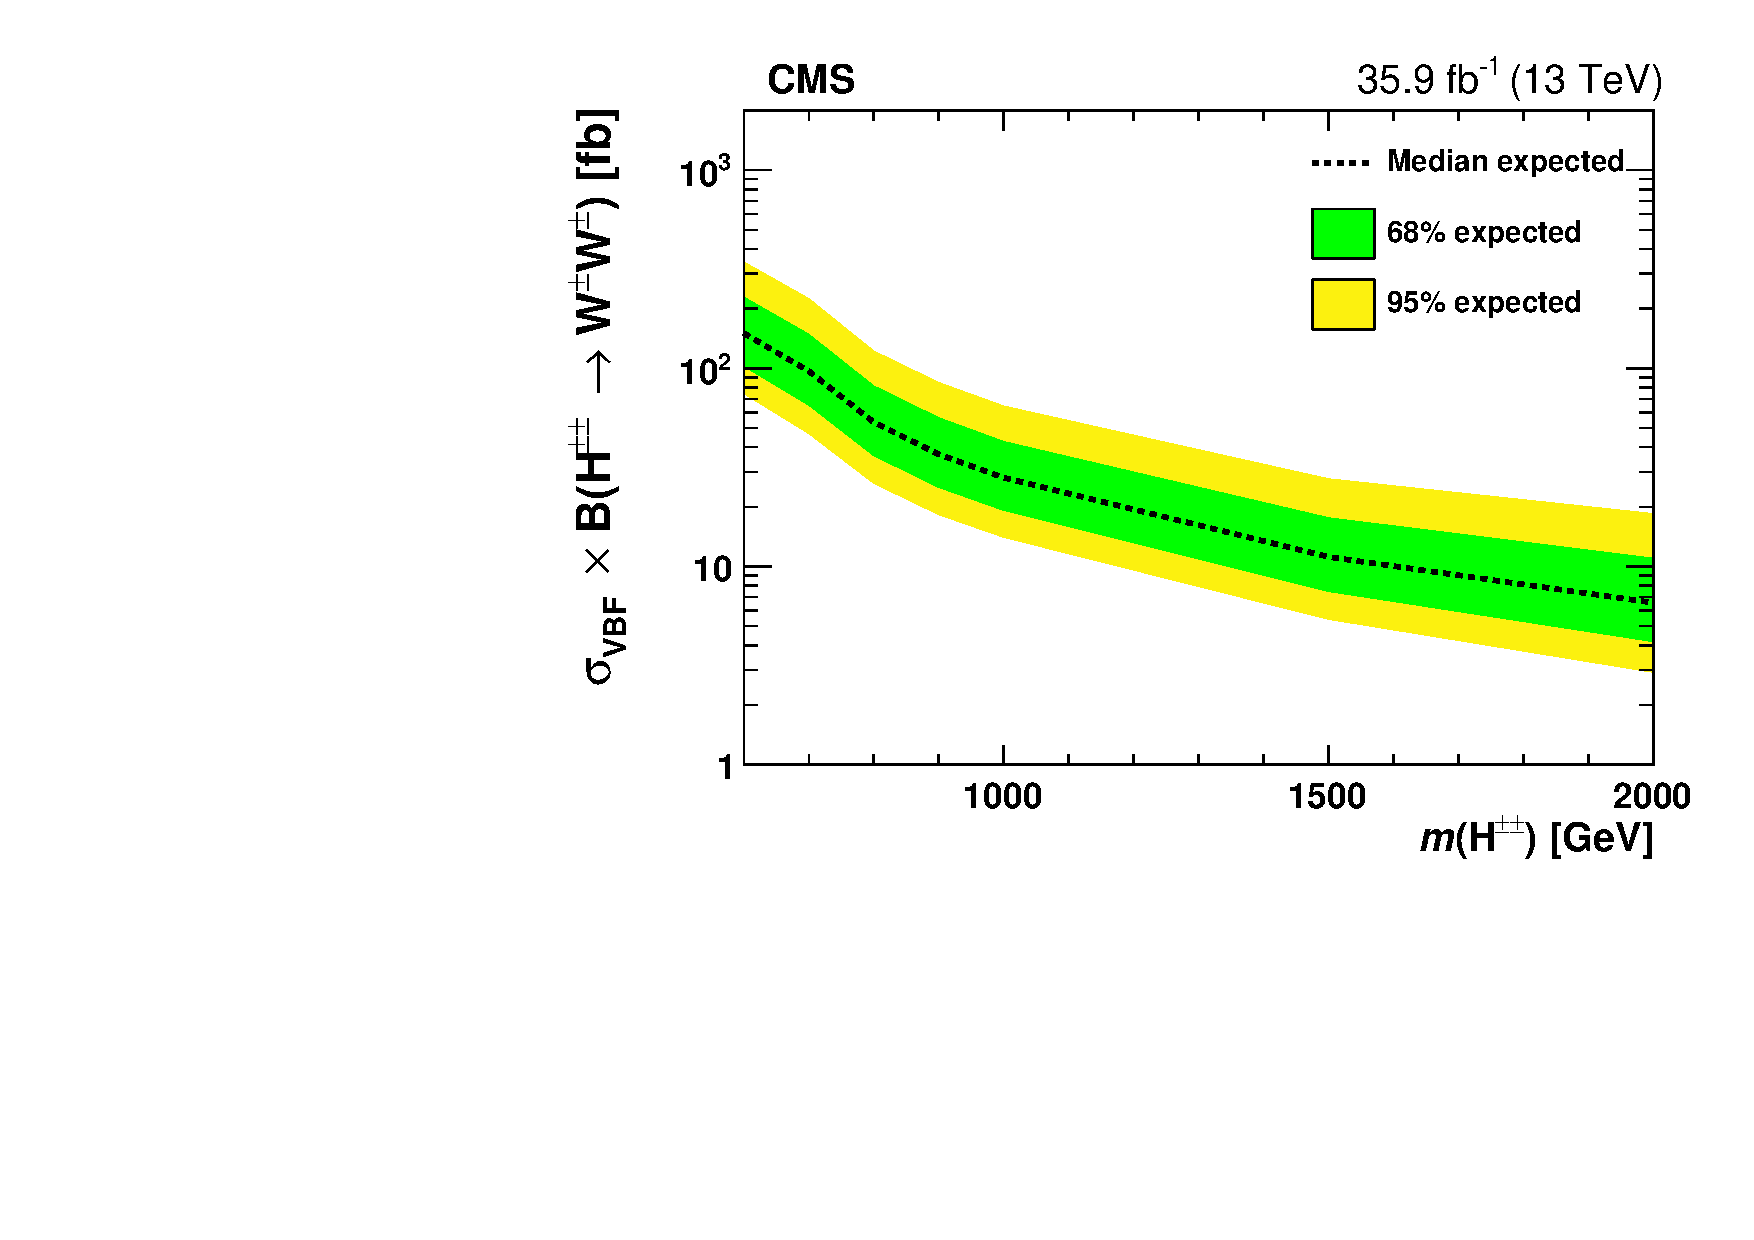
\includegraphics[width=0.45\textwidth]{Plots/plots/limits_wpwp.pdf}
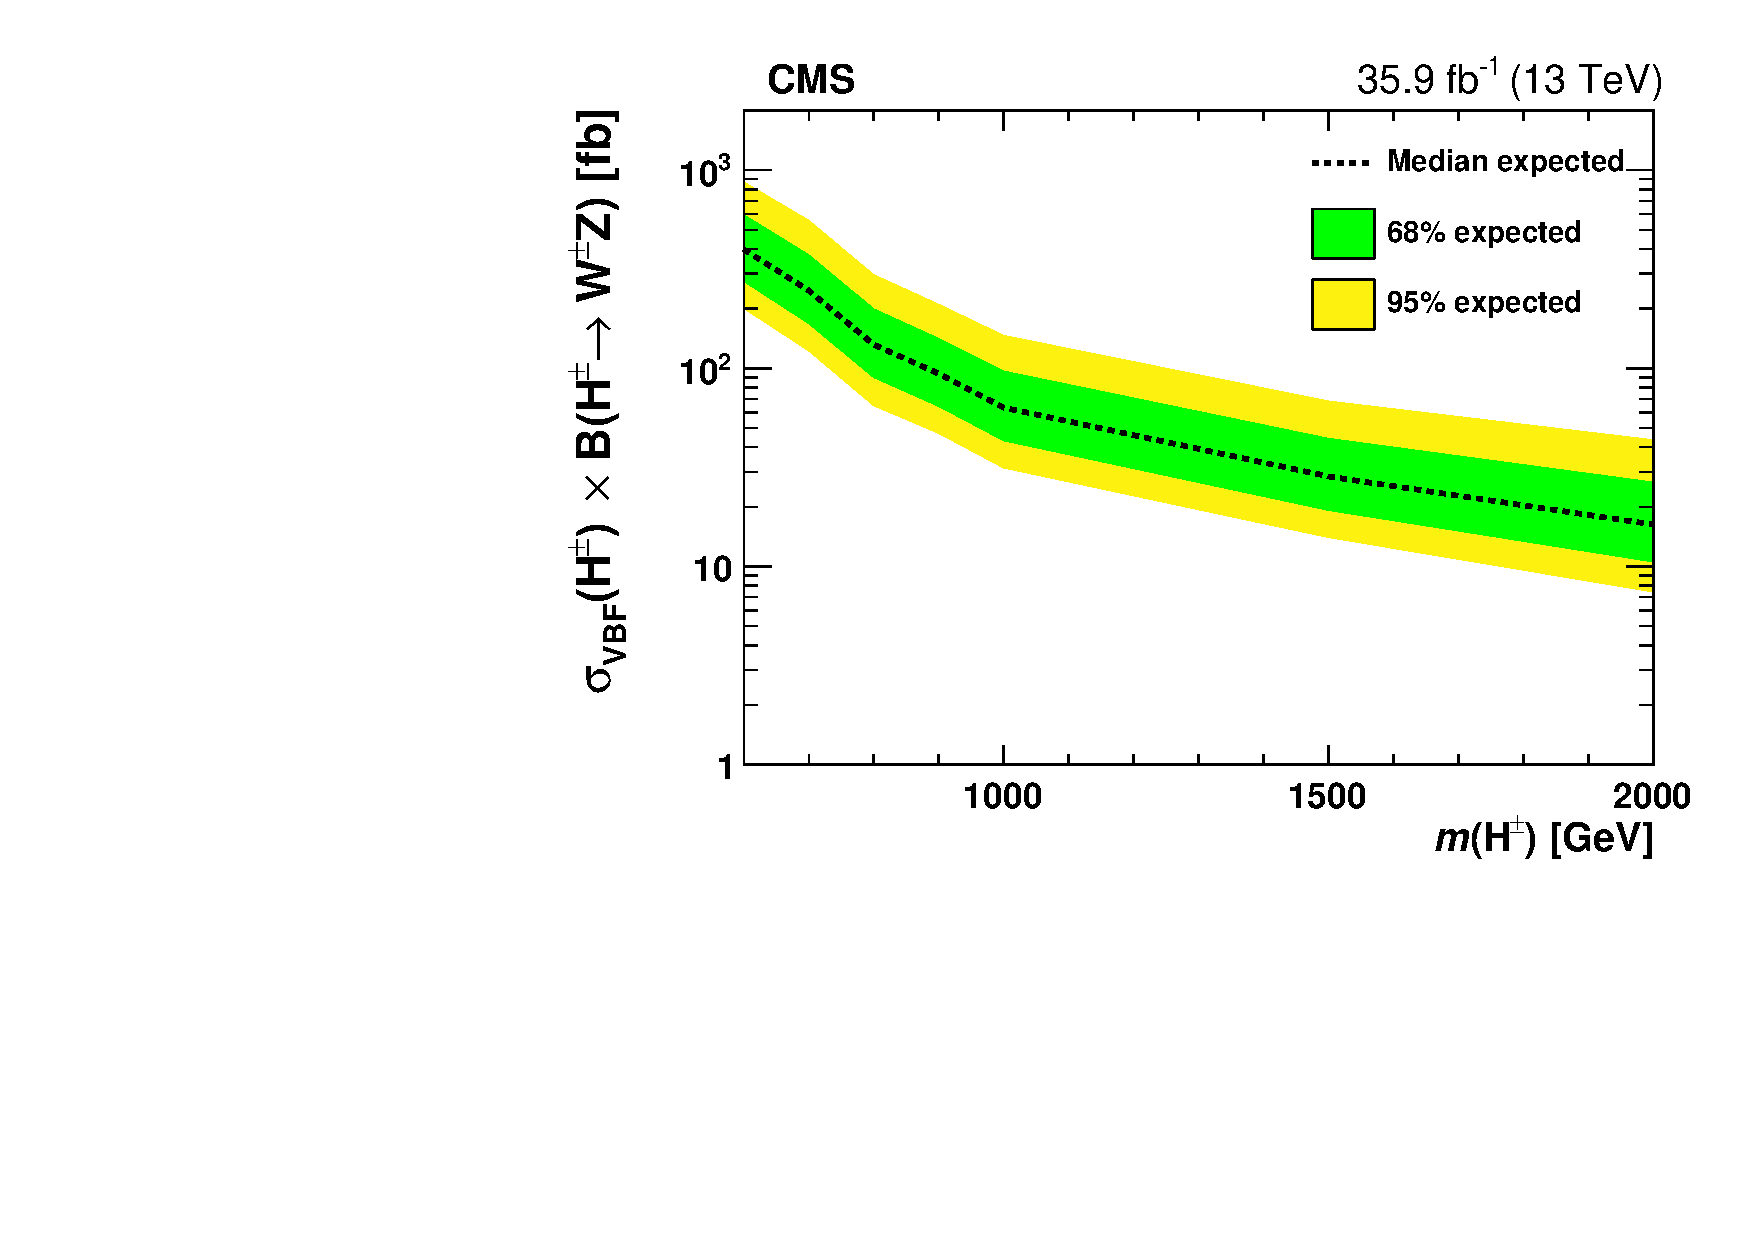
\includegraphics[width=0.45\textwidth]{Plots/plots/limits_wpz_lnu.pdf}
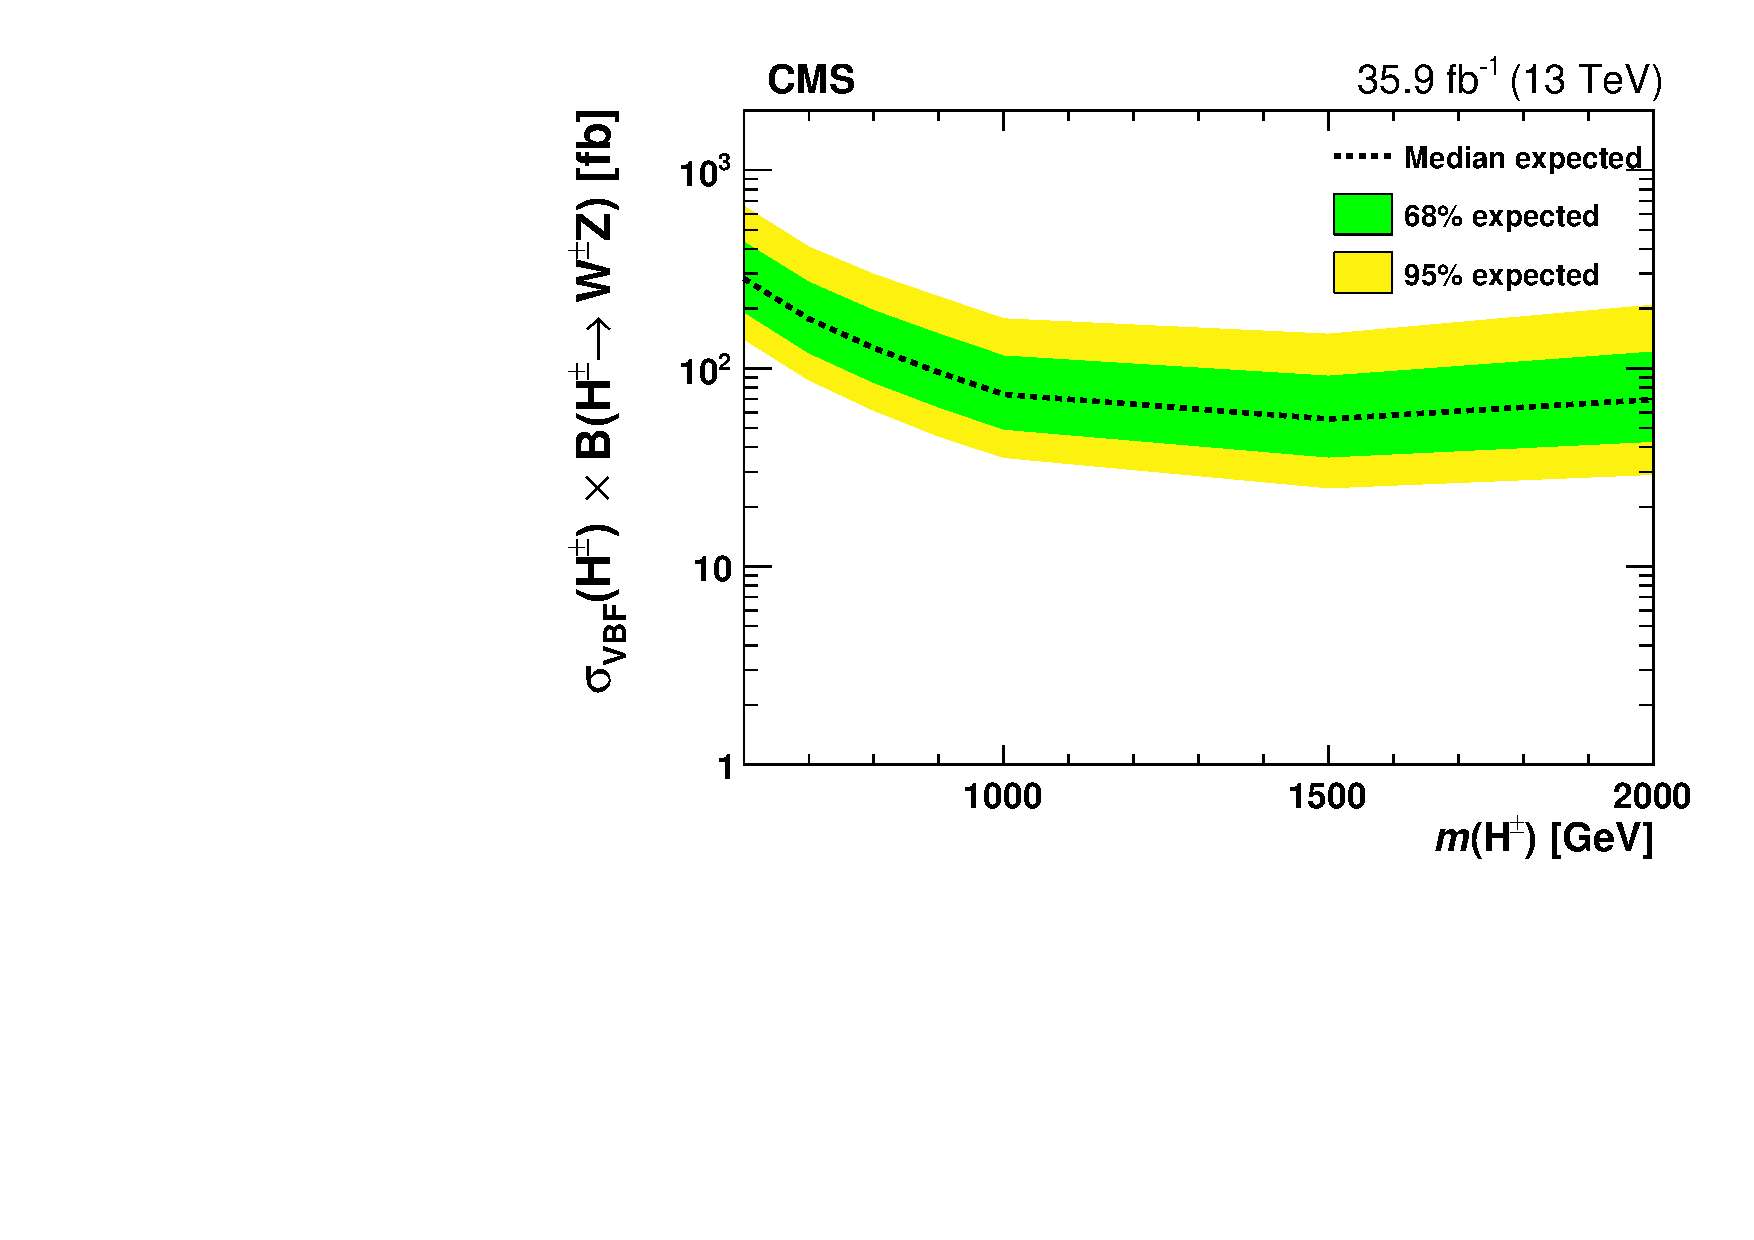
\includegraphics[width=0.45\textwidth]{Plots/plots/limits_wpz_ll.pdf}
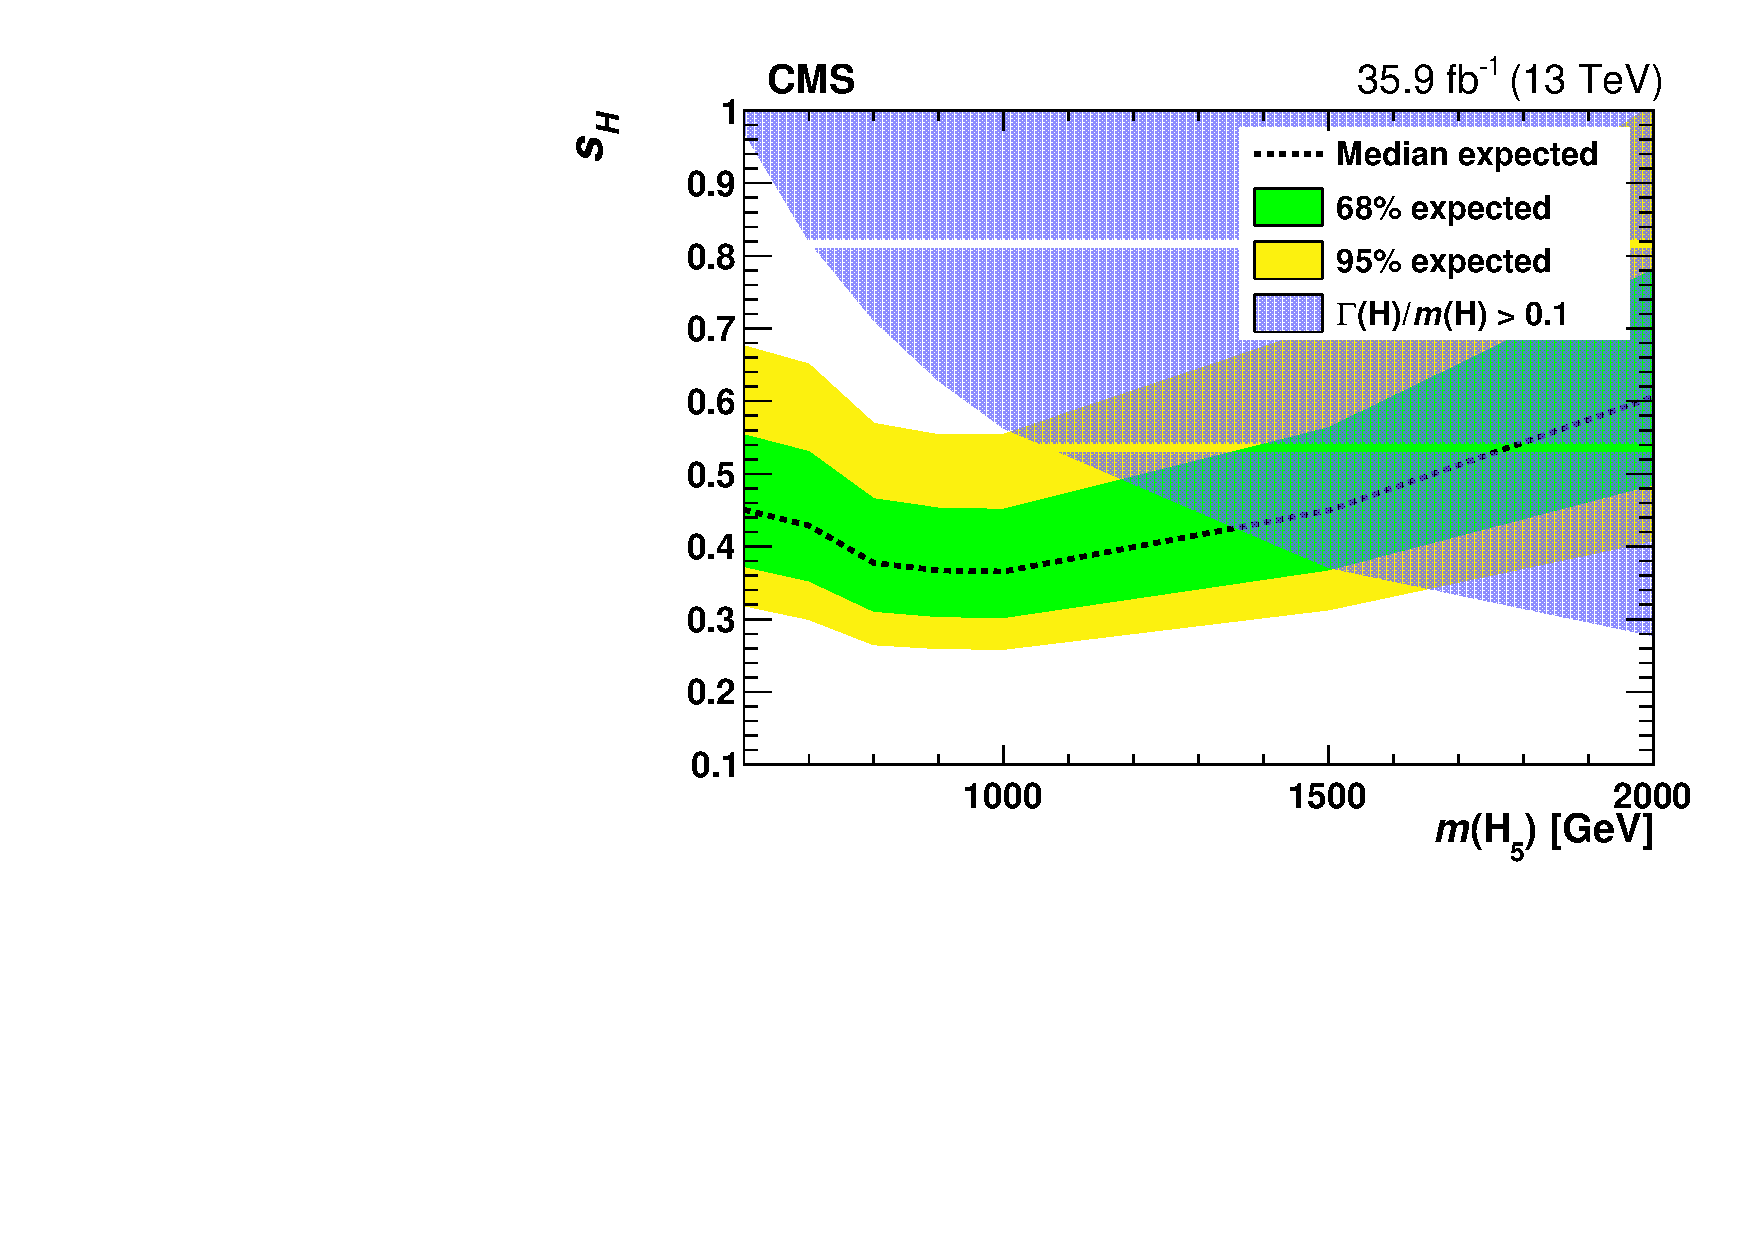
\includegraphics[width=0.45\textwidth]{Plots/plots/limits_model.pdf}
\caption{Expected and observed exclusion limits at 95\% confidence level as functions of $m(\PHpmpm)$ and $m(\PHpm)$ for $\sigma_\mathrm{VBF}(\PHpmpm) \, \mathcal{B}(\PHpmpm\to \PW\PW)$ (top left) and $\sigma_\mathrm{VBF}(\PHpm) \, \mathcal{B}(\PHpm\to \PW\Z)$ in the  $\PW V$ (top right) and $\PZ V$ (bottom left) final states, and on the ratio of vacuum expectation values in the GM model (bottom right). The blue shaded area covers the theoretically not allowed parameter space~\cite{Zaro:2002500}.
}
\label{fig:limits_s}
\end{figure}

\section{Future Outlook} % (fold)
\label{sec:future_outlook}
For future upgrades of the CMS detector to cope-up with the high luminosity runs of the LHC includes the upgrade of muon system. The CMS GEM community started R\&D of the GEM detectors for the CMS phase-II upgrade which  includes a  second GEM detector station (GE2/1) in the muon endcaps. This CMS GE2/1 upgrade will result  in increased  average number of muon hits registered in the muon detectors in the forward regions. The forwards regions of the CMS detector experience  high particle rates and and a low magnetic bending power and the addition of GEM detectors in these regions will, thus, improve the forward tracking. 
The CMS GEM collaboration is also working on the proposal for a MEO muon detector station for pseudo-rapidity regions lying between 2.2 to 2.8, for which the R\&D is also going on. 
The GEM foils produced in India, after passing the standard quality control criteria, will be used for these upgrades. The beam test studies performed during the course of this PhD thesis will be helpful to finalize the detector designs for these upgrades. The analysis framework developed could be employed during the data analysis of future beam test campaigns.  
Besides, the GEM detectors could also be used for the detection of ultra-violet and visible photons and studies are ongoing for their use in the medical industry~\cite{Wallmark2001,Tsyganov2008,Remillard2000} and for tomographic reconstruction~\cite{Gnanvo2010}. 

The physics analysis presented in this thesis marks the a starting phase of quartic-gauge coupling studies and the VBS at the LHC. Due to low values of production cross-section for the VBS processes, it has yet not been observed. In future, with refined analysis techniques and larger amount of data, it could be possible to improve the aQGC limits by several factors. The first step towards this goal would be to analyze complete LHC Run-II (2016-2018) data which correspond to an integrated luminosity of $\sim$150 $fb^{-1}$.
With this one might also be able to investigate the SM production of the electroweak process $W^+W^-jj$, which could be observed at least significance of 2-$\sigma$.
The Run-3 (2021-2023) of the LHC will be much more exciting for these kind of studies and should definitely provide yet more exciting information about the EWSB mechanism.
% section future_outlook (end)

% % chapter summary_&_outlook (end)